% SciTech 2027 final paper -- working draft.
% Scope note for the authors: the submitted extended abstract also promised ship-airwake results
% over multiple wind-over-deck conditions. Those are OUT of this paper (decision 2026-10-12); the
% paper covers the lid-driven cavity (Re 15k, 30k) and the Challenge 2.1 cavity PIV.
% Numbers in this draft come from results/*/saved_metrics, results/ldc_15k_dls_p99m10/
% reassembly_study_heldout.json and results/cavity_challenge_eval.json (scripts/challenge_eval.py).
% Red \todo{} marks results that are still running or not yet done.
\documentclass[conf]{new-aiaa}
\usepackage[utf8]{inputenc}

\usepackage{graphicx}
\usepackage{amsmath}
\usepackage{bm}
\usepackage{booktabs}
\usepackage{multirow}
\usepackage{xcolor}
\usepackage{siunitx}
\usepackage{longtable,tabularx}
\setlength\LTleft{0pt}

\graphicspath{{figs/}{../../figures/}{../lit_review/figs/}}
% keep floats near their text: looser placement limits, and no float crosses a section boundary
\usepackage[section]{placeins}
\renewcommand{\topfraction}{0.9}
\renewcommand{\bottomfraction}{0.8}
\renewcommand{\textfraction}{0.1}
\renewcommand{\floatpagefraction}{0.75}
\setcounter{totalnumber}{4}

\newcommand{\todo}[1]{\textcolor{red}{[TODO: #1]}}
\newcommand{\Rey}{\mathrm{Re}}
\newcommand{\dvec}{\mathbf{d}}
\newcommand{\dhat}{\hat{\mathbf{d}}}

\title{Localized Latent-Space Forecasting for Transformer-Based Turbulence Surrogates}

\author{Caleb A. Morton\footnote{Graduate Research Associate, Department of Mechanical \& Aerospace Engineering, morton.311@osu.edu, Student Member AIAA.} and Jack J. McNamara\footnote{Professor, Department of Mechanical \& Aerospace Engineering, mcnamara.190@osu.edu, Associate Fellow AIAA (Corresponding Author).}}
\affil{The Ohio State University, Columbus, Ohio, 43210}
\author{Rohit Deshmukh\footnote{Assistant Professor, Department of Mechanical \& Aerospace Engineering, rohit.deshmukh@ucf.edu.}}
\affil{University of Central Florida, Orlando, Florida, 32816}

\begin{document}

\maketitle

\begin{abstract}
Transformer surrogates for turbulent flows are usually trained on a single global latent vector per time step, so the network must learn correlations across the whole domain at once. We instead use a data-enriched finite element basis, the Data-informed Local Subspace (DLS), as a tokenizer: each finite element of a coarse mesh becomes one token that carries its local enrichment coefficients, and a transformer attends across elements to forecast every element's next state. Treating the latent space as a finite element space has two consequences that we exploit. First, the element mass (Gram) matrix gives the physical energy of any latent error, and we use it in both the training loss and the evaluation. Second, independently predicted elements must be reassembled into a conforming field, and we show that a mass-weighted projection, built from the element mass matrices, does this better than the nodal averaging used previously, particularly when it is applied inside the training rollout. For the lid-driven cavity at a Reynolds number of 15,000, with four times fewer latent coefficients than our prior work, the model's mean 30-step relative field error over 50 held-out forecasts is 3.8\%, against 32.4\% for persistence. Its 500-step root-mean-square velocity field is within 1.4 percentage points of the compression floor, and these results are consistent across three random seeds. At a Reynolds number of 30,000 the same recipe overfits a short, bursty training record. A longer record raises the 30-step skill over persistence from 0.02 to 0.33, but the long rollout still loses a third of its energy, and weight decay and input noise do not help. On the Challenge 2.1 cavity PIV, scored with the official metric on held-out sequences, a 1.9-million-parameter version of the model reaches a mean 30-step normalized mean-square error of 0.78, against 1.09 for the dynamic mode decomposition baseline and 1.0 for the mean flow, and stays below the mean-flow forecast at every lead time.
\end{abstract}

\section*{Nomenclature}

{\renewcommand\arraystretch{1.0}
\noindent\begin{longtable*}{@{}l @{\quad=\quad} l@{}}
$\mathbf{B}$ & element basis matrix, local DLS shape functions sampled on the element's grid points \\
$\dvec$, $\dvec_e$ & global and element-local latent coefficient (DOF) vectors \\
$\dhat_e$ & element-local coefficients predicted by the network \\
$E$ & number of finite elements (tokens) \\
$\mathbf{G}_e$ & Boolean gather matrix, $\dvec_e = \mathbf{G}_e\dvec$ \\
$H$ & forecast horizon, steps \\
$\mathbf{M}_e$, $\mathbf{M}$ & element and assembled mass (Gram) matrices of the DLS basis \\
$m$ & number of local POD enrichment modes per node \\
$N_i$ & bilinear finite element shape function of node $i$ \\
$n_\mathrm{skip}$ & grid points between finite element nodes \\
$\Rey$ & Reynolds number \\
$S$ & forecast skill relative to persistence \\
$\mathbf{u}'$ & fluctuating velocity field \\
$\mathbf{W}$, $\mathbf{W}_e$ & diagonal grid-point weights of an element (zero outside the domain for cut elements) \\
$\varepsilon_k$ & relative field error after $k$ forecast steps \\
$\lambda$ & regularization of the assembly and loss metrics \\
$\tau$ & number of input snapshots (context length) \\
$\psi_k$ & $k$th local POD enrichment mode
\end{longtable*}}

%=====================================================================================
\section{Introduction}
\lettrine{D}{ata-driven} surrogate models are an attractive way to accelerate the analysis and prediction of turbulent flows. High-fidelity simulations and time-resolved measurements produce datasets that are expensive to generate, store, and analyze, and the cost of the underlying computation becomes prohibitive in many-query settings such as design studies, uncertainty quantification, and real-time or control-oriented applications \cite{benner2015survey}. A common strategy is to first compress each snapshot into a low-dimensional latent state and then learn the evolution of that state. Compression makes learning tractable: the number of trainable parameters, the amount of data required, and the cost of each forecast step all scale with the latent dimension rather than with the number of grid points \cite{brunton2020ml,vinuesa2022enhancing,brunton2024promising}.

Most reduced-order models compress with global modal decompositions such as proper orthogonal decomposition (POD) \cite{sirovich1987,berkooz1993,holmes2012turbulence,taira2017modal,taira2020modal}. Global modes are effective when a few energetic coherent structures dominate the flow. Their performance degrades for high-Reynolds-number turbulence with a wide range of spatial scales, for convection-dominated flows \cite{mojgani2017lagrangian}, and when operating conditions change \cite{deshmukh2016sparse}. Correlations in turbulent flows decay with separation, so a global mode that represents a structure in one region spends degrees of freedom everywhere else. Localized representations avoid this. Earlier approaches treated difficult regions separately \cite{lucia2001thesis}, built local bases in state space \cite{amsallem2012local}, or decomposed the domain into subdomains with their own bases \cite{hoang2021ddlspg,diaz2024ddnm}. The Data-informed Local Subspace (DLS) method of Deshmukh et al.~\cite{deshmukh2020dls} combines the generalized finite element method (GFEM) \cite{melenk1996pum,babuska2004gfem} with local POD modes learned from snapshot data. The result is a compactly supported, $C^0$-continuous basis that reuses the same small set of local modes everywhere in the domain.

Neural-network autoencoders offer nonlinear compression \cite{gonzalez2018deep,lee2020cae,eivazi2022betavae}, and recurrent networks \cite{srinivasan2019,eivazi2021koopman,borrelli2022channels,vlachas2020backprop}, Koopman embeddings \cite{lusch2018koopman}, and transformers \cite{vaswani2017attention} have all been used to evolve the resulting latent states. Transformers capture long-range temporal dependencies without recurrence. Wu et al.~\cite{wu2022transformer} paired them with POD, Solera-Rico et al.~\cite{solera2024betavae} with $\beta$-variational autoencoders, and Geneva and Zabaras \cite{geneva2022transformers} with Koopman embeddings; Hemmasian and Barati Farimani \cite{hemmasian2023transformers} and Sarma et al.~\cite{sarma2024tbl} applied them to turbulent datasets. Almost all of these models forecast one global latent vector per time step. Autoregressive forecasting of turbulence remains difficult because errors compound over the rollout, the dynamics are chaotic, and the latent state may not be closed (Markovian) after truncation \cite{lusch2018koopman,linot2023stabilized,kohl2023acdm,lippe2023pderefiner}.

Finite element spaces have also entered learned surrogates. Operator networks such as FEONet \cite{lee2025feonet} and its discontinuous Galerkin extension \cite{chawla2026dgfeonet}, which works element by element, predict finite element coefficients and train without data on the residual of a weak form; they target parametric PDEs rather than time-series forecasting. Mesh-informed neural networks \cite{franco2023minn} embed their hidden layers in finite element spaces for operator learning. For unsteady flows, Gao et al.~\cite{gao2024hypergraph} pass messages through the elements of a simulation mesh and roll the model out in time, and Lu et al.~\cite{lu2026graphrom} compress with a finite-element-inspired graph autoencoder and forecast with a spatiotemporal transformer. Local reduced bases have also been paired with networks, which have been trained to predict the local basis functions and coarse matrices of multiscale finite elements \cite{wang2019gmsfem} and the POD coefficients of each subdomain of a decomposed domain \cite{pan2024ddpdcnn}. We are not aware of a learned forecasting model, other than our earlier work \cite{morton2026scitech}, whose latent state is the coefficient vector of a data-enriched finite element basis.

Our previous work \cite{morton2026scitech} trained transformers on DLS and POD latent spaces of a lid-driven cavity at Reynolds numbers of 15,000 and 30,000. DLS latents preserved long-time turbulence statistics better than POD latents of comparable size. However, the root-mean-square (RMS) velocity error grew by an order of magnitude between the two Reynolds numbers, from 2.1\% to 15.3\%, and a simple frequency-domain extrapolation of the latent coefficients matched the transformer (1.7\% and 10.1\%). That study localized the representation but not the forecast. The transformer still received the entire latent vector, 10,648 coefficients for $49\times49$ patches with ten local modes, and predicted all of it at once.

This paper poses the forecast locally. A DLS latent state is a set of finite elements, each with its own coefficients and a known position. We therefore treat each element as one token, in the same way that vision transformers tokenize image patches \cite{dosovitskiy2021vit} and that recent neural surrogates tokenize spatial locations or latent anchors \cite{serrano2024aroma,alkin2024upt}. A transformer attends across the element tokens and predicts each element's next state. This also sets a consistent goal for the representation. The latent space is used as a tokenization for a purely data-driven, attention-based model; no governing equations enter the forecast. The finite element structure is retained, however, because it supplies two things a generic tokenizer does not: an exact energy metric on the latent space, and an assembly operator that turns independent element predictions into one conforming field.

The energy metric is not new in itself. The $L^2$ norm of a finite element function is a quadratic form in its coefficients through the mass matrix, and the same weighted inner product is used to compute POD from finite element snapshots \cite{parish2023residual}. Mesh-informed networks \cite{franco2023minn} and a recent domain-decomposed reduced model for steady elliptic problems \cite{dimola2026ddrom} train on this norm of finite element fields, and the latitude-weighted loss of GraphCast \cite{lam2023graphcast} is its analogue with a diagonal metric. In the orthonormal POD coefficients used by most reduced-order surrogates the metric is the identity, so a Euclidean loss already measures field energy. What differs here is the space it acts on. The DLS latent state is compressed, enriched, and far from orthogonal, so the mass matrix is severely ill-conditioned and a Euclidean loss on the coefficients is badly misaligned with field energy (Sec.~\ref{sec:gram}). The metric must then be regularized, and it is evaluated directly on the coefficients during an autoregressive rollout, without decoding the field.

We also move to stronger compression. The latent spaces used here have 2,662 and 1,452 coefficients, four and seven times fewer than in Ref.~\cite{morton2026scitech}. The compression error then sets a floor on every statistic. We report that floor alongside every result, so that forecasting error and compression error can be separated.

Finally, we follow recommended evaluation practice for machine learning on fluid problems \cite{mcgreivy2024weak}. All headline numbers are on a contiguous held-out time window. We compare against persistence, report the spread across many independent short forecasts, and repeat the headline recipes over three random seeds. The short-horizon protocol mirrors the forecasting track of the community challenge of Schmidt et al.~\cite{schmidt2026challenge}, which asks for 30-step forecasts and scores the mean and the spread across test sequences.

The contributions of this paper are:
\begin{enumerate}
  \item an element-token formulation of latent forecasting on a data-enriched finite element basis, with attention over space and one token per element;
  \item the use of the DLS mass (Gram) matrix as the metric for both the training loss and the evaluation of a forecasting model in a compressed, non-orthogonal latent space, together with a demonstration that the raw coefficient metric is badly misaligned with field energy;
  \item a mass-weighted projection that assembles independently predicted elements and includes nodal averaging as a limiting case, and training through this assembly inside a multi-step rollout;
  \item a fictitious-domain extension of the DLS mesh that represents grids whose size is not a multiple of the element size, removing the truncation of the original construction;
  \item a held-out, multi-start, multi-seed evaluation with persistence and compression-floor references; and
  \item results at substantially higher compression for the lid-driven cavity at two Reynolds numbers and for the Challenge 2.1 cavity PIV.
\end{enumerate}

%=====================================================================================
\section{Data-Informed Local Subspace Latent Space}
\label{sec:dls}

\subsection{Construction}
DLS \cite{deshmukh2020dls} embeds data-driven local modes in a GFEM approximation \cite{melenk1996pum,babuska2004gfem}. A coarse mesh of bilinear finite elements, with nodes every $n_\mathrm{skip}$ grid points, is laid over the data grid. Its shape functions $N_i$ form a partition of unity, and each $N_i$ is supported on the patch $\omega_i$ of the elements that share node $i$. Patches of $(2n_\mathrm{skip}+1)^2$ grid points are sampled at random locations from a single training snapshot (the first of the record), their means are removed, and POD of the sampled patches gives $m$ local modes $\psi_k$. Because the local modes need only one snapshot, the basis never sees the held-out data. The same modes are used at every node, centered on the node so that their footprint covers $\omega_i$. The fluctuating velocity is then approximated as
\begin{equation}
  \mathbf{u}'(\mathbf{x},t)\approx\sum_{i}N_i(\mathbf{x})\Bigl[a_i(t)+\sum_{k=1}^{m}b_{ik}(t)\,\psi_k(\mathbf{x}-\mathbf{x}_i)\Bigr],
  \label{eq:gfem}
\end{equation}
separately for each velocity component. Each enrichment $N_i\psi_k$ vanishes on the boundary of $\omega_i$, so the representation is $C^0$-continuous. Every node therefore carries $m+1$ coefficients per component. The coefficients of a snapshot are obtained by $L^2$ projection onto the enriched space, i.e., by assembling and solving the global system $\mathbf{M}\dvec=\mathbf{P}$, where $\mathbf{P}$ is the projection of the snapshot onto the basis \cite{deshmukh2020dls}. Figure~\ref{fig:dls} illustrates the construction in one dimension.

\begin{figure}[!tbp]
  \centering
  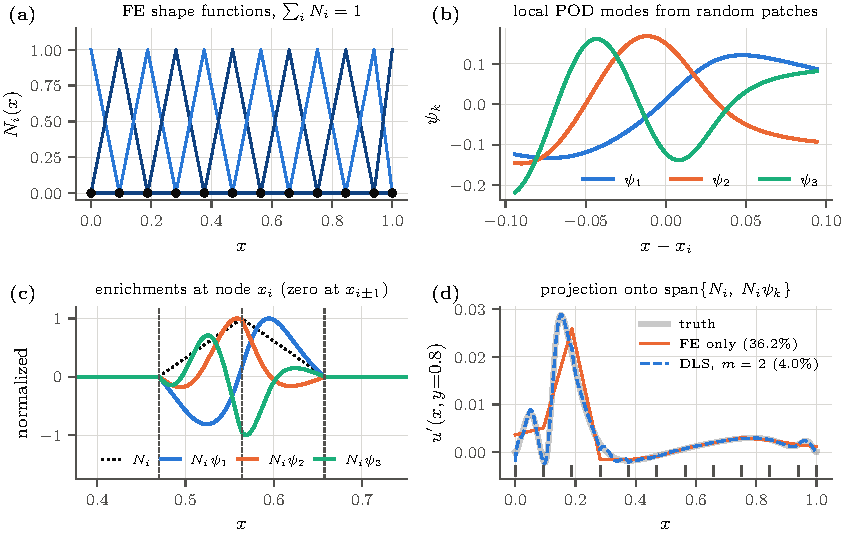
\includegraphics[width=0.85\textwidth]{dls_schematic.pdf}
  \caption{DLS construction in one dimension. (a) Finite element shape functions forming a partition of unity. (b) Local POD modes obtained from randomly sampled patches. (c) Enrichments $N_i\psi_k$ at one node; they vanish at the neighboring nodes. (d) Projection of a cavity velocity profile onto the shape functions alone and onto the enriched space.}
  \label{fig:dls}
\end{figure}

\subsection{Element-local structure and the field-energy metric}
\label{sec:gram}
The reconstruction is linear and block-diagonal by element. Let $\dvec_e=\mathbf{G}_e\dvec$ gather the $n_e=4(m+1)$ coefficients per component of the four nodes of element $e$. The field over the element is then $\mathbf{u}_e=\mathbf{B}\dvec_e$. Here $\mathbf{B}$ holds the products $N_i\psi_k$ sampled on the element's grid points, and it is the same for every element of a uniform mesh. Grid points on shared element edges and corners are weighted by a diagonal matrix $\mathbf{W}$ that splits them among the elements that contain them. The field energy of any coefficient vector is then exactly
\begin{equation}
  \|\mathbf{u}\|^2=\sum_{e=1}^{E}\dvec_e^{\top}\mathbf{M}_e\dvec_e=\dvec^{\top}\mathbf{M}\dvec,\qquad
  \mathbf{M}_e=\mathbf{B}^{\top}\mathbf{W}\mathbf{B},\qquad
  \mathbf{M}=\sum_{e}\mathbf{G}_e^{\top}\mathbf{M}_e\mathbf{G}_e .
  \label{eq:gram}
\end{equation}
The coefficients therefore live in the $\mathbf{M}$ metric, not the Euclidean one. The distinction is large in practice. For the production basis used below, $\mathbf{B}$ has a condition number of $3.2\times10^{5}$ and the assembled $\mathbf{M}$ has a condition number of $2.5\times10^{10}$. Many coefficient directions carry almost no field energy, and a mean-squared error on raw coefficients is dominated by them. For real model errors, the gradient of a mean-squared error on the standardized coefficients lies $83$--$86^\circ$ from the gradient of the field-energy error, on both bases used below. It still descends, because $\mathbf{M}$ is positive semidefinite, but very inefficiently.

We use Eq.~\eqref{eq:gram} in three places. The training loss scores the element errors in a regularized element metric,
\begin{equation}
  \mathcal{L}=\frac{1}{H_\mathrm{tr}}\sum_{k=1}^{H_\mathrm{tr}}\sum_{e=1}^{E}\bigl\|\mathbf{R}_\lambda\bigl(\dhat_e^{(k)}-\dvec_e^{(k)}\bigr)\bigr\|^2,\qquad
  \mathbf{R}_\lambda=\Bigl(\mathbf{M}_e+\lambda\,\tfrac{\operatorname{tr}\mathbf{M}_e}{n_e}\mathbf{I}\Bigr)^{1/2},
  \label{eq:loss}
\end{equation}
summed over both velocity components. With $\lambda=0$ this is exactly the field energy of the error. The ridge is needed because the near-null directions of $\mathbf{M}_e$ are invisible in the field but are fed back to the network as inputs. With $\lambda=0$ nothing constrains them, and they drift during autoregressive rollouts. A smaller ridge is not enough either: at $\Rey=15{,}000$, a model trained with $\lambda=10^{-6}$ had a step-30 error of 0.065, against 0.035--0.037 for three seeds at $\lambda=10^{-2}$, and its 500-step rollout grew to 21 times the true energy. \todo{Revise with the ridge sweep (full-coverage $\alpha=0.1$ basis, $\Rey=15{,}000$). Seed 1, $\lambda=10^{-2}$, $10^{-3}$, $10^{-4}$, $10^{-5}$, $10^{-6}$: 30-step mean error 0.0276, 0.0223, 0.0153, 0.0219, 0.0330; 500-step RMS error 6.2, 6.5, 7.0, 47, 171\%; TKE error 1.3, 2.3, 3.9, 82, 729\%; final energy 1.02, 1.00, 0.93, 3.4, 21. Three seeds at $10^{-4}$ against $10^{-2}$: $0.0172\pm0.0028$ against $0.0271\pm0.0008$, RMS $8.4\pm1.8$\% against $6.27\pm0.05$\%, TKE $5.0\pm1.3$\% against $1.6\pm0.3$\%. Smaller $\lambda$ improves the short horizon down to $10^{-4}$ while the long-run statistics worsen steadily; below $10^{-4}$ the rollout grows. On Challenge 2.1, $\lambda=0$--$10^{-3}$ show no consistent NMSE change. Decide which $\lambda$ the paper uses, or present the trade-off as a figure.} With $\lambda=10^{-2}$ the weakest coefficient direction has a relative weight of $3.5\times10^{-4}$ instead of $4\times10^{-11}$.
The ridge is not a small correction, however. The true coefficients are large along the ill-conditioned directions, because a modest field component along such a direction needs a large coefficient. At $\lambda=10^{-2}$ the ridge therefore carries 99.8\% of the metric norm of the true $\Rey=15{,}000$ coefficients and 97\% of the norm of the forecast errors. For the better-conditioned Challenge 2.1 basis (Sec.~\ref{sec:challenge}), it carries 77\% and 85--91\%. The gradient of Eq.~\eqref{eq:loss} lies $75$--$81^\circ$ from the field-energy gradient for $\Rey=15{,}000$ model errors, and $39$--$51^\circ$ for Challenge 2.1 model errors. The loss is therefore the field-energy error plus a penalty on the coefficients, and on the lid-driven cavity the penalty is most of the loss. Terms that should act on the visible field alone, such as the energy term of Sec.~\ref{sec:tradeoff}, are therefore computed with $\lambda=0$, in the same units. The unregularized metric scores forecast errors in Sec.~\ref{sec:eval}, and the regularized one, with the same $\lambda$, defines the assembly in Sec.~\ref{sec:assembly}. Evaluating Eq.~\eqref{eq:gram} costs one $n_e\times n_e$ product per element, so no field needs to be decoded.

A side result illustrates the point. POD computed directly on the stored coefficients, using the snapshot correlation $\mathbf{D}^{\top}\mathbf{M}\mathbf{D}$ in place of $\mathbf{D}^{\top}\mathbf{D}$, reproduces POD of the full $491\times491$ field for the cavity: the energy fractions agree to $5\times10^{-4}$, and the principal angles between the leading 20-mode subspaces are zero to four digits. The cost scales with the 1,331 coefficients per component instead of the 241,081 grid points, and the eigenproblem is solved 14 times faster. POD on the raw coefficients instead misorders the modes (minimum principal cosine 0.23 for five modes). \todo{Decide whether to keep this paragraph; it supports the metric argument and is cheap, but is tangential to forecasting.}

\subsection{Covering the whole grid}
\label{sec:fullcover}
A uniform mesh with nodes every $n_\mathrm{skip}$ grid points covers an $n_x\times n_y$ grid only when $n_x-1$ and $n_y-1$ are multiples of $n_\mathrm{skip}$. Otherwise the trailing rows and columns lie outside every element and are dropped. For the production lid-driven cavity mesh this is a 21-point strip along the right wall and along the lid; for the Challenge 2.1 grid it is 3 columns and 2 rows. We remove the truncation with a fictitious-domain construction. Wherever the grid would be truncated, one more row or column of nodes is added past the edge, so the last elements overhang the domain. Grid points outside the domain carry zero weight: element $e$ uses $\mathbf{W}_e=\mathbf{W}\,\mathrm{diag}(\mathbf{m}_e)$, where $\mathbf{m}_e$ is 1 at the element's points inside the domain and 0 elsewhere. Every use of the mass matrix then takes the element's own $\mathbf{M}_e=\mathbf{B}^{\top}\mathbf{W}_e\mathbf{B}$: the compression solve, the loss and error metrics of Eqs.~\eqref{eq:loss} and \eqref{eq:err}, and the assembly of Sec.~\ref{sec:assembly}. Only a few distinct masks occur (interior, right column, top row, corner), so the extra cost is negligible. Nodes past the edge are observed only through the few grid points their support shares with the domain, so the compression solve adds a ridge of $10^{-8}$ times the mean diagonal of $\mathbf{M}$.

On the Challenge 2.1 grid, the extended mesh has 234 elements instead of 200 and 3,240 coefficients instead of 2,808, and it represents all $154\times51$ points. Its compression floor over the held-out block is the same as the truncated mesh's over the region that mesh covers (normalized mean-square error 0.036). The new strip alone is represented less accurately (0.061), as expected for elements observed only in part. The masked metric reproduces the in-domain field energy exactly, whereas applying the uncut element metric to the cut elements would overcount it by 48\%. The lid-driven cavity results in this paper use the original mesh, and all of their errors and compression floors are computed on the $491\times491$ region it covers. \todo{Re-run the $\Rey=15{,}000$ headline recipe on a full-coverage basis, so the lid strip is included.}

\subsection{Latent spaces considered}
Table~\ref{tab:latent} lists the bases. Both production bases use $99\times99$ patches ($n_\mathrm{skip}=49$), which on the $512\times512$ cavity grid gives a $10\times10$ element mesh covering $491\times491$ grid points. With $m=10$ local modes, the latent state has 2,662 coefficients; with $m=5$ it has 1,452. The basis of Ref.~\cite{morton2026scitech} used $49\times49$ patches and ten modes, for 10,648 coefficients. The compression floor is the RMS-velocity error of the DLS reconstruction of the true snapshots over the evaluation window. It bounds what any forecast in that latent space can achieve.

\begin{table}[!tbp]
  \centering
  \small
  \caption{DLS latent spaces for the lid-driven cavity at $\Rey=15{,}000$.}
  \label{tab:latent}
  \begin{tabular}{lccccccc}
    \toprule
    Basis & Patch & $m$ & Nodes & Elements & Coefficients & Points per coefficient\textsuperscript{a} & RMS floor, \% \\
    \midrule
    Ref.~\cite{morton2026scitech} & $49^2$ & 10 & $22\times22$ & 441 & 10,648 & 48 & 0.6 \\
    p99m10 (this work) & $99^2$ & 10 & $11\times11$ & 100 & 2,662 & 181 & 4.28 \\
    p99m5 (this work)  & $99^2$ & 5  & $11\times11$ & 100 & 1,452 & 332 & 8.84 \\
    \bottomrule
  \end{tabular}

  \smallskip
  {\footnotesize \textsuperscript{a}Grid points covered by the mesh per coefficient of one velocity component.}
\end{table}

%=====================================================================================
\section{Forecasting on Element Tokens}
\label{sec:model}

\subsection{Spatial transformer}
Each of the $E=100$ elements becomes one token. The token holds the element's coefficients for both velocity components over the last $\tau=4$ snapshots, $2n_e\tau=352$ values for p99m10. Each coefficient is standardized over the training set. A linear layer projects the token to the model width $d=256$. A Fourier-feature embedding of the element centroid \cite{tancik2020fourier}, with six octave-spaced frequencies per coordinate, is added to it. Four pre-normalized \cite{xiong2020layer} transformer encoder layers with four heads and SwiGLU feed-forward blocks of width 768 \cite{shazeer2020glu} then attend across all elements. A final normalization and linear head map each token to its element's next-step coefficients. The head predicts a residual: its output is added to the most recent input frame, and its weights are initialized to zero, so the untrained model is persistence. The model has 7.48 million parameters. For the Challenge 2.1 cavity we also use a narrower version (width 128, feed-forward width 384; 1.88 million parameters), which forecasts as well as the full one (Sec.~\ref{sec:res_challenge}).

Time enters only through the stacked frames in each token, and attention runs over space. Because no attention runs across time, the model needs no temporal positional encoding such as rotary embeddings \cite{su2024roformer}. Element position is supplied by the coordinate embedding. Every element attends to every other, so each local prediction can draw on the state of the whole cavity. What is local is the representation: each output is the update of one element's coefficients, and the same weights are shared by all elements. Figure~\ref{fig:arch} summarizes one step of the forecast, including the assembly described next.

\begin{figure}[!tbp]
  \centering
  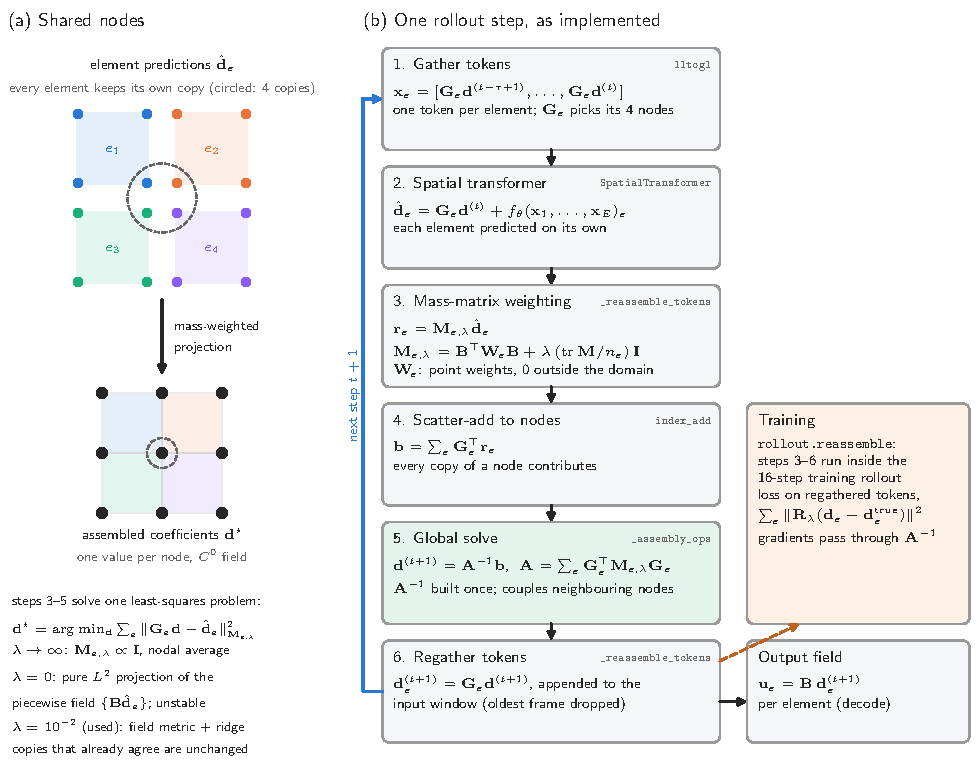
\includegraphics[width=\textwidth]{assembly_schematic.pdf}
  \caption{Element-token forecasting with mass-weighted projection. (a) Each element predicts its own copy of every node it touches (exploded view; the circled node has four copies). The mass-weighted projection returns one value per node, so the field is continuous. (b) One rollout step as implemented: element tokens are gathered from the nodal coefficients, the spatial transformer predicts each element, the predictions are weighted by each element's mass matrix, scattered to the nodes and solved for one global coefficient vector, which is regathered and fed back. In training, steps 3--6 run inside the rollout and the loss scores the regathered tokens.}
  \label{fig:arch}
\end{figure}

\subsection{Assembling element predictions}
\label{sec:assembly}
Each node is shared by up to four elements, and each of those elements predicts the node's coefficients independently. The predictions are not identical, so they must be combined into one global coefficient vector before the next step. If they are not, the copies drift apart. Figure~\ref{fig:reassembly}a shows the mismatch at shared nodes in a rollout without assembly: it grows to 44\% of the predicted frame's energy by step 500. The original formulation averaged each node's copies. This is least squares in the raw coefficient metric, which, as shown in Sec.~\ref{sec:gram}, is not the metric of the field.

Finite element assembly instead projects the discontinuous element-wise field onto the conforming space in the field metric. We use a regularized version,
\begin{equation}
  \dvec^{\star}=\arg\min_{\dvec}\sum_{e}\bigl(\mathbf{G}_e\dvec-\dhat_e\bigr)^{\top}\mathbf{M}_{e,\lambda}\bigl(\mathbf{G}_e\dvec-\dhat_e\bigr)
  \;\Longrightarrow\;
  \Bigl(\sum_{e}\mathbf{G}_e^{\top}\mathbf{M}_{e,\lambda}\mathbf{G}_e\Bigr)\dvec^{\star}=\sum_{e}\mathbf{G}_e^{\top}\mathbf{M}_{e,\lambda}\dhat_e,
  \label{eq:assembly}
\end{equation}
with $\mathbf{M}_{e,\lambda}=\mathbf{M}_e+\lambda\,(\operatorname{tr}\mathbf{M}_e/n_e)\,\mathbf{I}$. We call Eq.~\eqref{eq:assembly} the mass-weighted projection. It projects the predicted field onto the DLS space; unlike the Galerkin projection of POD-based reduced-order models, it involves no governing equations. The family contains both existing choices. As $\lambda\rightarrow\infty$ the metric becomes the identity, and Eq.~\eqref{eq:assembly} reduces to the nodal average. With $\lambda=0$ it is the pure $L^2$ projection, which decodes each element and re-encodes the field. The pure $L^2$ projection is unstable in a rollout. The near-null directions of $\mathbf{M}$ are almost free under the field metric, so the projection injects large coefficients along them; these are invisible in the field but feed back through the network's inputs. Intermediate values of $\lambda$ remove inter-element disagreement in the field metric while keeping a floor under every direction. We use $\lambda=10^{-2}$, the same value as in the loss. On a full-coverage mesh (Sec.~\ref{sec:fullcover}) each cut element uses its own $\mathbf{M}_e$, and every ridge is scaled by the trace of a full element, so the weakly observed coefficients of cut elements are held as firmly as interior ones. The left-hand matrix of Eq.~\eqref{eq:assembly} is fixed, so its inverse is computed once (1,331 unknowns per velocity component for p99m10). Each step then costs one matrix--vector product per component, a negligible fraction of a transformer forward pass, and the whole operation is linear and therefore differentiable.

The operation itself is classical. A global least-squares projection of discontinuous element-wise data onto a continuous nodal field is the standard way to recover smooth stresses from displacement-based finite element solutions, where it is compared with nodal averaging \cite{oden1971consistent,hinton1974smoothing,zienkiewicz1992spr}. Nodal averaging replaces the mass matrix with the identity, in the spirit of mass lumping \cite{hinton1976lumping,hughes2000fem}, although for enriched coefficients the identity is not a lumped mass matrix in the usual sense. The ridge term is a Tikhonov regularization \cite{tikhonov1977illposed,hoerl1970ridge}. In learned mesh-based models, nodes duplicated on element boundaries have so far been reconciled by averaging their values or features \cite{barwey2024consistent,sankaran2025elementlocal}, and domain-decomposed POD surrogates average their solutions where subdomains meet \cite{pan2024ddpdcnn}. Local learned and reduced models have also been coupled through interface constraints or Schwarz iterations \cite{diaz2024ddnm,heinlein2021ddml}. Separately, Kinch et al.~\cite{kinch2026hybridizable} embed an autoregressive transformer in a mixed finite element discretization in time. To our knowledge, a mass-weighted projection has not previously been used to combine learned element predictions, nor has a surrogate been trained through one.

The assembly can be applied only at inference, or inside the training rollout as well. In the second case the loss scores the assembled state, and the network is trained on the consistent states it receives at inference. Both variants are evaluated in Sec.~\ref{sec:res_assembly}.

\subsection{Training}
The model is trained by free-running multi-step rollouts. Each training sample is a window of $\tau+H_\mathrm{tr}$ consecutive snapshots with $H_\mathrm{tr}=16$. The model is seeded with the first $\tau$ true frames and then fed its own (assembled) predictions. The loss of Eq.~\eqref{eq:loss} is accumulated at every step. Gradients propagate through the rollout by truncated backpropagation through time \cite{werbos1990} in chunks of eight steps, with gradient checkpointing \cite{chen2016checkpoint} to keep memory constant in the rollout depth. The backpropagation depth grows from one step to eight over the first 20 epochs, because a freshly initialized model rolled out many steps produces non-finite gradients. Training on multi-step rollouts, rather than single steps, is known to improve the stability of autoregressive neural surrogates \cite{brandstetter2022mpnn,vlachas2020backprop}, and Sec.~\ref{sec:res_training} confirms that it is essential here.

We use Adam \cite{kingma2015adam} with a learning rate of $10^{-3}$, halved after five epochs without improvement on the test split, batches of 64 windows, gradient clipping at a norm of one, and mixed precision. Training stops when the test loss has not improved by 1\% for ten epochs. On the $\Rey=15{,}000$ data this takes 73--102 epochs and under 70 minutes on a single NVIDIA RTX 3090 Ti. Early stopping and the learning-rate schedule can optionally be held until the depth ramp ends, so that a run is not stopped while its objective is still deepening. On the Challenge 2.1 data this made no difference, because the held-out loss reached its minimum before the ramp ended. For the regularization study at $\Rey=30{,}000$ we also use AdamW \cite{loshchilov2019adamw}, with decoupled weight decay applied to weight matrices only.

%=====================================================================================
\section{Evaluation Protocol}
\label{sec:eval}

\subsection{Held-out split}
Each record is split into three contiguous blocks in time: training $[0,a)$, test $[a,b)$, and evaluation $[b,T)$. The evaluation block holds the last 20\% of the record, the test block the preceding 10\% of the remainder, and the training block everything before it. Every training window lies entirely in the training block, and every test window in the test block. The test block is used only for early stopping and learning-rate control, and the evaluation block is never seen during training or model selection. For the $\Rey=15{,}000$ cavity, training windows cover snapshots 0--1799, test windows 1800--1998, and evaluation 1999--2498. \todo{Footnote or appendix note: the architecture and training-recipe studies of Secs.~\ref{sec:res_arch}--\ref{sec:res_training} used an earlier split in which the early-stopping windows overlapped training data; the evaluation window was held out in both. Re-running the headline recipes on the corrected split changed their skill by less than 0.01 (0.853$\pm$0.005 to 0.861$\pm$0.010, and 0.885$\pm$0.009 to 0.883$\pm$0.005), so the earlier rankings stand. Re-run those studies on the corrected split for the final version.}

\subsection{Short-horizon forecasts}
A single long rollout starts from one initial condition, so any spread it shows is over time steps, not over forecasts. We therefore launch $N_s=50$ forecasts of $H=30$ steps from starting points spread evenly across the evaluation block. Each forecast is seeded with $\tau$ true frames. The error after $k$ steps is the relative field error
\begin{equation}
  \varepsilon_k=\frac{\|\dhat^{(k)}-\dvec^{(k)}\|_{\mathbf{M}}}{\|\dvec^{(k)}\|_{\mathbf{M}}},\qquad \|\dvec\|_{\mathbf{M}}^2=\dvec^{\top}\mathbf{M}\dvec ,
  \label{eq:err}
\end{equation}
where $\dvec^{(k)}$ is the DLS projection of the true fluctuating field. Through Eq.~\eqref{eq:gram} this is the exact field-space $L^2$ error. We verified it against full $491\times491$ reconstructions, which agreed to a median of 0.36\%. Because the reference is the projected truth, $\varepsilon_k$ measures forecasting error alone; compression error is reported separately as the floor in Table~\ref{tab:latent}. We report the mean of $\varepsilon_k$ over forecasts and steps, $\bar\varepsilon$, the per-step mean and spread, and the standard deviation across forecasts of each forecast's window-mean error, $\sigma_\mathrm{start}$. The challenge's normalized mean-square error \cite{schmidt2026challenge} is $\varepsilon_k^2$ evaluated on the challenge's own field.

Persistence, which holds the last seed frame, is the reference. On this cavity the field changes by about 2.1\% per snapshot, so persistence scores $\varepsilon_1=0.021$ and $\varepsilon_{30}=0.62$, and any forecast with a one-step error near 0.1 is worse than doing nothing. The skill is $S=1-\bar\varepsilon/\bar\varepsilon_\mathrm{persist}$: $S=0$ is persistence and $S=1$ is a perfect forecast.

\subsection{Long-horizon statistics}
Beyond the 30-step window, each model is rolled out freely for 496 steps from the start of the evaluation block (about five convective time units). The predicted coefficients are decoded, and we compare the following against the original data: the RMS velocity field, the turbulent kinetic energy (TKE) time history, the ratio of predicted to true fluctuating energy, and velocity spectra and probability densities at probes. RMS and TKE errors are relative $L^2$ errors against the DNS. They therefore include the compression floor.

An RMS or TKE error mixes amplitude, location, and scale, and it gives no indication of how close two records of the same flow can be. For the Challenge 2.1 cavity we therefore also compare the free rollout and the true flow over the same block using five statistics, each chosen to isolate one property of the fluctuating velocity:
\begin{enumerate}
  \item the energy ratio, the mean predicted-to-true fluctuating energy (amplitude);
  \item the relative $L^2$ error of the RMS-velocity map (where the fluctuations are);
  \item the log-spectral distance, in decibels, between the streamwise wavenumber spectra, each normalized by its total and summed in octave bands (how the energy is distributed across spatial scales, with amplitude removed);
  \item the same distance for the frequency spectra, computed by Welch's method at every fourth grid point, which contain the Rossiter tones (the distribution across time scales);
  \item the Wasserstein-1 distance between one-point velocity distributions after each record is standardized by its own local standard deviation, averaged over grid points (the shape of the distribution, including skewness and tails, with amplitude removed).
\end{enumerate}
None of these depends on timing, so a forecast is not penalized for losing phase with the truth. Each distance is divided by a sampling floor: the mean distance between the held-out truth and eight equally long segments of the training record. A ratio of 1 means that the forecast is as close to the truth as another stretch of the true flow. The floors themselves vary across segments by 9\% (distribution shape) to 51\% (spatial spectrum) of their means, so ratios below about 2 do not separate models. The DLS projection of the truth gives a second reference, the closest that any forecast in that basis can come. \todo{Compute the same measures for the lid-driven cavity rollouts (floors from segments of the training record).}

\subsection{Seeds}
Headline recipes are trained with three random seeds, which change the weight initialization, the dropout masks, and the order of the training windows. We report the mean $\pm$ one standard deviation across seeds. Run-to-run differences from nondeterministic GPU kernels are about $10^{-7}$ in $\bar\varepsilon$ and are negligible.

%=====================================================================================
\section{Flow Configurations}
\label{sec:flows}

\subsection{Lid-driven cavity}
The lid-driven cavity data are from direct numerical simulation of the nondimensional incompressible Navier--Stokes equations in a unit square, discretized on a $512\times512$ uniform grid, at $\Rey=15{,}000$ and $30{,}000$ \cite{deshmukh2016sparse,morton2026scitech}. Both records are sampled at 100 snapshots per nondimensional time unit. The $\Rey=15{,}000$ record has 2,499 snapshots. The $\Rey=30{,}000$ record has 60,000 snapshots. We use its first 4,500 and first 10,000 snapshots and compress only the snapshots that are used, so the 10,000-snapshot study also changes the length of the evaluation block. \todo{Cite the original DNS reference used in Ref.~\cite{morton2026scitech} (its refs.\ 22 and 32).}

\subsection{Challenge 2.1 cavity PIV}
\label{sec:challenge}
The second dataset is the time-resolved PIV of a Mach 0.6 open-cavity flow by Zhang et al.~\cite{zhang2020samm}, used in Challenge 2.1 of the community challenge \cite{schmidt2026challenge}. The cavity has a length-to-depth ratio of 6, and the Reynolds number based on its depth is about $3.3\times10^5$. The field of view is resolved by $154\times51$ points, and the snapshots are sampled at 16~kHz. The flow combines broadband turbulence, Rossiter tones, and measurement noise. Of the 16,000 snapshots, 12,800 are released for training. The remaining 3,200 form 32 test sequences of 100 snapshots; the first 70 snapshots of each are given, and the last 30 must be forecast. The official metric is the per-step normalized mean-square error (NMSE) of the mean-removed field, $\mathbb{E}\|\hat{\mathbf{q}}_k-\mathbf{q}_k\|^2/\mathbb{E}\|\mathbf{q}_k\|^2$, reported as the mean and standard deviation across sequences. The challenge baselines are dynamic mode decomposition (DMD) \cite{schmid2010dmd} with 25 modes fit to each sequence's 70 inputs, and an LSTM on 25 global POD coefficients.

We split the 12,800 training snapshots as in Sec.~\ref{sec:eval}, with the last 10\% held out: training windows lie in snapshots 0--10,367, test windows in 10,368--11,519, and evaluation in 11,520--12,799. The basis uses $13\times13$ patches ($n_\mathrm{skip}=6$) and five local modes. With the full-coverage mesh of Sec.~\ref{sec:fullcover} it has $27\times10$ nodes, 234 elements, and 3,240 coefficients, and its compression floor over the held-out block is an NMSE of 0.036. With the original mesh and the uncovered strip set to the mean flow, the floor is 0.042.

%=====================================================================================
\section{Results}
\label{sec:results}

\subsection{Global versus element-token forecasting}
\label{sec:res_arch}
Table~\ref{tab:arch} compares three architectures on the same p99m10 latent space, all trained with the field-energy loss and 16-step rollouts. The global temporal transformer, like Ref.~\cite{morton2026scitech}, treats the whole 2,662-coefficient vector as one token per time step and attends over 16 past steps. The global--local encoder--decoder encodes the element tokens of the most recent frame into a shared context and attends over time within each element. The spatial transformer of Sec.~\ref{sec:model} attends over elements only.

The element-token models forecast best over 30 steps. The spatial transformer improves on the global model in every metric, with a 30-step error of 0.072 against 0.125 and an RMS error of 6.9\% against 9.3\%, while using a larger but still modest network. The encoder--decoder has good short-horizon skill, but its long rollout gains energy (TKE error 28\%), so we do not pursue it further. The global model starts with a first-step error of 0.062, three times that of persistence, and its error then stays nearly flat near 0.055 for several steps; it beats persistence only from the third step. Both element-token models beat persistence from the first step.

\begin{table}[!tbp]
  \centering
  \small
  \caption{Architecture comparison, $\Rey=15{,}000$, p99m10, single seed, nodal-average assembly. Persistence: $\bar\varepsilon=0.324$, $\varepsilon_{1}=0.021$, $\varepsilon_{30}=0.621$.}
  \label{tab:arch}
  \begin{tabular}{lccccccc}
    \toprule
    Model & Parameters & Attention over & $S$ & $\varepsilon_{1}$ & $\varepsilon_{30}$ & RMS error, \% & TKE error, \% \\
    \midrule
    Global temporal transformer & 2.53 M & time (16 steps) & 0.740 & 0.062 & 0.125 & 9.31 & 15.3 \\
    Global--local enc.--dec.\textsuperscript{a} & 8.23 M & elements, then time & 0.822 & 0.009 & 0.101 & 36.9 & 28.2 \\
    Spatial transformer & 7.48 M & elements & 0.854 & 0.006 & 0.072 & 6.94 & 1.85 \\
    \bottomrule
  \end{tabular}

  \smallskip
  {\footnotesize \textsuperscript{a}Trained with the additional trajectory penalties of Table~\ref{tab:training}.}
\end{table}

\todo{Add a POD latent with the same spatial-transformer-equivalent capacity, and the frequency-extrapolation baseline of Ref.~\cite{morton2026scitech}, to Table~\ref{tab:arch}; both were promised implicitly by the comparison to prior work and are expected by reviewers \cite{mcgreivy2024weak}. Report wall-clock cost per forecast step for the global and element-token models.}

\subsection{Training recipe}
\label{sec:res_training}
Table~\ref{tab:training} varies the training recipe of the spatial transformer. Teacher-forced one-step training, with a single input frame, gives an accurate first step but diverges in the long rollout: by the end of the window the fluctuating energy has grown 570-fold. Multi-step training is therefore essential. Adding penalties on the trajectory's energy, variance, and time derivative (each with weight 0.1) degraded the 30-step error and made the long rollout gain energy. A longer 30-step training horizon with input noise, combined with the same penalties, reduced the 30-step skill further while giving a stable long-run energy. The plain field-energy loss with 16-step rollouts is the best of these recipes, and we use it from here on.

\begin{table}[!tbp]
  \centering
  \caption{Training-recipe ablation for the spatial transformer, $\Rey=15{,}000$, p99m10, single seed, nodal-average assembly. Energy ratio is the mean predicted-to-true fluctuating energy over the 496-step rollout.}
  \label{tab:training}
  \begin{tabular}{lccccc}
    \toprule
    Recipe & $S$ & $\varepsilon_{1}$ & $\varepsilon_{30}$ & RMS error, \% & Energy ratio \\
    \midrule
    One-step, $\tau=1$ & 0.633 & 0.008 & 0.229 & 2351 & 570 \\
    16-step rollout (baseline) & 0.854 & 0.006 & 0.072 & 6.94 & 0.99 \\
    \quad + trajectory penalties & 0.772 & 0.008 & 0.130 & 123 & 3.24 \\
    30-step rollout + input noise + trajectory penalties & 0.613 & 0.040 & 0.150 & 9.26 & 0.96 \\
    \bottomrule
  \end{tabular}
\end{table}

\subsection{Assembly of element predictions}
\label{sec:res_assembly}
Table~\ref{tab:assembly} and Fig.~\ref{fig:reassembly} compare four ways of combining the element predictions, each over three seeds on the held-out split. In the first three rows the same trained weights are used, and only the inference-time assembly changes.

Without assembly, the 30-step skill is unchanged ($S=0.860$), but the copies of shared nodes drift apart. Their disagreement grows from $3\times10^{-5}$ to 44\% of the frame energy over 500 steps (Fig.~\ref{fig:reassembly}a), and the RMS error triples to 18.2\%. Short-horizon skill is therefore a poor guide to whether a model is fit for long forecasts. Nodal averaging holds the disagreement near $5\times10^{-5}$ and reduces the RMS error to 6.25\%.

The mass-weighted projection, applied to the same weights, improves every metric. The skill rises from 0.861 to 0.879, the 30-step error falls from 0.068 to 0.059, and the RMS error falls from 6.25\% to 5.74\%. The improvement holds in every seed. Training through the projection adds a smaller further gain, concentrated in the 30-step error ($0.053\pm0.001$) and in the consistency across seeds: the seed spread of the skill halves, and that of the 30-step error falls by a factor of three. The RMS error, 5.64\%, is 1.4 percentage points above the 4.28\% compression floor, against 2.0 points for nodal averaging.

Figure~\ref{fig:assembly_example} shows what the projection does to real predictions, 30 steps into a held-out rollout. A model trained through the projection learns to rely on it. Before the global solve, its element outputs disagree along shared edges by 125\% of the field's RMS value, and the patchwork field is 28\% from the truth; after the solve the edges agree to round-off and the error is 4.3\%. Because the loss only ever sees the projected state, the network is free to place content in the directions that the projection removes, and its raw output is an intermediate rather than a forecast. A model trained on raw outputs produces nearly consistent elements (edge jumps of 1.2\%), and the projection barely changes its error at a single step (4.7\% before and after). For that model, the projection's benefit is that it stops the slow drift of Fig.~\ref{fig:reassembly}a.

The improvement is not uniform across statistics. The TKE error of the model trained through the projection is $2.11\pm0.46$\%, against $1.78\pm0.38$\% for nodal averaging; the ranges overlap. Its mean energy ratio is $1.007\pm0.008$, against $0.994\pm0.002$. \todo{Small $\lambda$ sweep figure or table (inference-only: $\lambda=0$ diverges; $10^{-2}$--$1$ beats the mean; $\lambda\to\infty$ recovers it), re-run on the held-out split.}

\begin{table}[!tbp]
  \centering
  \small
  \caption{Assembly study, $\Rey=15{,}000$, p99m10, held-out split, mean $\pm$ standard deviation over three seeds. Compression floor for the RMS error: 4.28\%. Persistence: $\bar\varepsilon=0.324$, $\varepsilon_{30}=0.621$.}
  \label{tab:assembly}
  \begin{tabular}{llcccc}
    \toprule
    Assembly at inference & Trained with & $S$ & $\bar\varepsilon$ & $\varepsilon_{30}$ & RMS error, \% \\
    \midrule
    None & raw outputs & $0.860\pm0.010$ & $0.045\pm0.003$ & $0.072\pm0.005$ & $18.2\pm0.7$ \\
    Nodal average & raw outputs & $0.861\pm0.010$ & $0.045\pm0.003$ & $0.068\pm0.004$ & $6.25\pm0.26$ \\
    Mass-weighted, $\lambda=10^{-2}$ & raw outputs & $0.879\pm0.010$ & $0.039\pm0.003$ & $0.059\pm0.004$ & $5.74\pm0.11$ \\
    Mass-weighted, $\lambda=10^{-2}$ & projection in the loop & $0.883\pm0.005$ & $0.038\pm0.002$ & $0.053\pm0.001$ & $5.64\pm0.09$ \\
    \bottomrule
  \end{tabular}
\end{table}

\begin{figure}[!tbp]
  \centering
  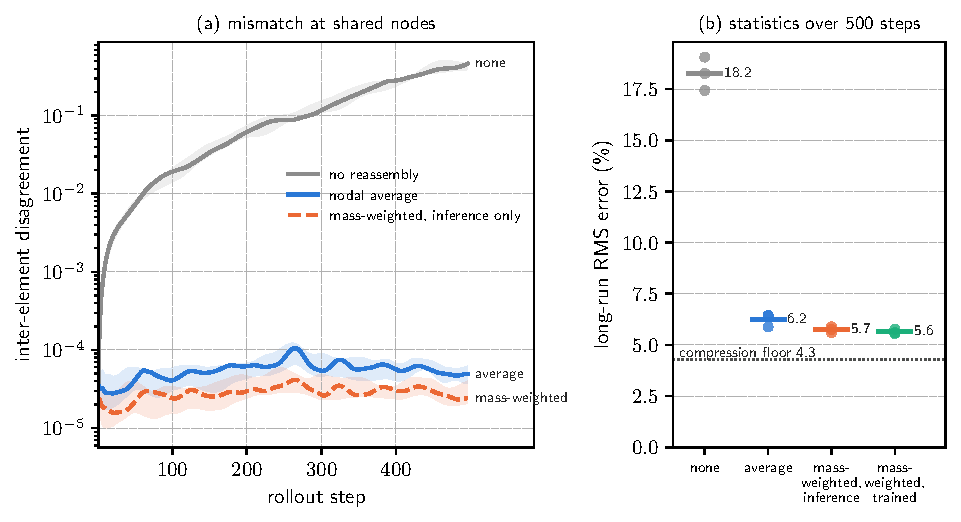
\includegraphics[width=\textwidth]{reassembly_study.pdf}
  \caption{Assembly of element predictions, $\Rey=15{,}000$, three seeds per setting. (a) Disagreement between elements at shared nodes during the 496-step rollout, as a fraction of the predicted frame's field energy (mean and seed range). (b) RMS velocity error over the rollout for each seed (dots) and the mean (bars); the dotted line is the compression floor.}
  \label{fig:reassembly}
\end{figure}

\begin{figure}[!tbp]
  \centering
  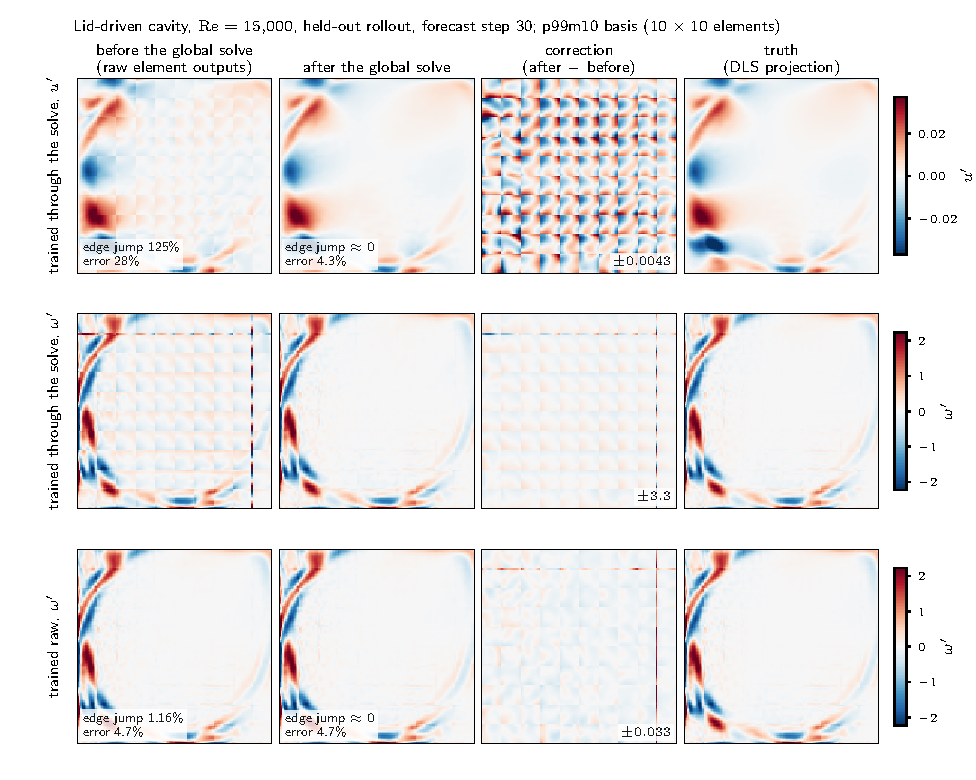
\includegraphics[width=\textwidth]{assembly_example.pdf}
  \caption{Element predictions before and after the global solve, $\Rey=15{,}000$, step 30 of a held-out rollout (seed 1). Columns: raw element outputs, each element decoded on its own; the field after the mass-weighted projection; the correction applied by the solve, on its own color scale ($\pm$ value shown); and the DLS projection of the truth. Rows: a model trained through the solve, streamwise velocity and vorticity; a model trained on raw outputs, vorticity. Edge jump is the RMS mismatch between neighboring elements along their shared edges, relative to the RMS of the velocity field; error is the relative velocity error against the projected truth.}
  \label{fig:assembly_example}
\end{figure}

\subsection{Short-horizon forecasts}
\label{sec:res_short}
Figure~\ref{fig:multistart} shows the per-step error of the 150 held-out forecasts (50 per seed) for nodal averaging and for the model trained through the mass-weighted projection. Both models stay well below persistence throughout. Their errors are 3.4--3.7 times smaller at the first step and 9--12 times smaller at step 30, where they reach 0.068 and 0.053 against 0.62 for persistence. Over the window, the model trained through the projection has a mean error of 0.038, a skill of 0.883, and a forecast-to-forecast spread of $\sigma_\mathrm{start}=0.0035$. The two recipes cross at step four. The model trained through the projection is slightly less accurate at the first step (0.0062 against 0.0057), and its advantage grows thereafter. This is consistent with a projection that removes some of the network's one-step detail but keeps errors from compounding. In terms of the challenge metric, a 30-step relative error of 0.053 is a normalized mean-square error of $2.8\times10^{-3}$.

\begin{figure}[!tbp]
  \centering
  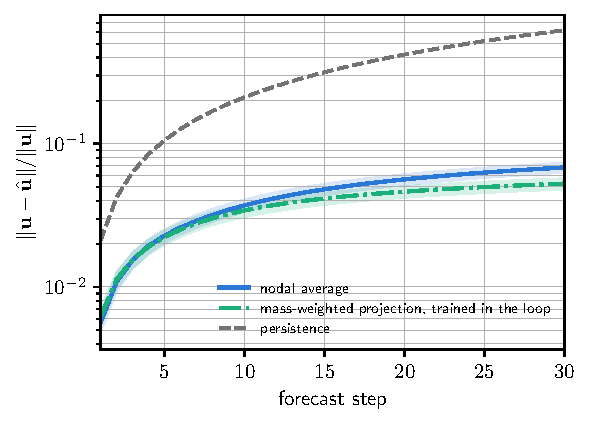
\includegraphics[width=0.6\textwidth]{multistart_heldout.pdf}
  \caption{Relative field error of 30-step forecasts from 50 evenly spaced held-out starts for each of three seeds, $\Rey=15{,}000$, p99m10. Lines are means over the 150 forecasts and bands are $\pm$ one standard deviation. Persistence holds the last seed frame.}
  \label{fig:multistart}
\end{figure}

\subsection{Long-horizon statistics}
\label{sec:res_long}
\todo{Figure: RMS $u$ and $v$ fields (truth, DLS reconstruction, nodal average, projection in the loop), TKE time history over the 496-step rollout, and probe PSDs, for seed 1. These exist per run in results/*/figs and need a combined paper figure.} Over the 496-step rollout, the model trained through the projection keeps the fluctuating energy within 1\% of the truth on average ($1.007\pm0.008$). The probability density of the velocity has a standard deviation within 0.4\% of the truth, and the RMS error is $5.64\pm0.09$\% against a floor of 4.28\%. Reference~\cite{morton2026scitech} reported RMS errors of $\mathcal{O}(1\%)$ at this Reynolds number with a basis whose own floor was 0.6\%. The present model works with four times fewer coefficients and a seven-times-higher floor, and it adds 1.4 percentage points to that floor. \todo{Decide how to present this comparison fairly, since the 2026 split and basis differ; consider re-evaluating the 2026 model with the present protocol.}

\subsection{Compression level}
\label{sec:res_compression}
Table~\ref{tab:compression} repeats the recipe with five local modes (1,452 coefficients). The short-horizon errors are smaller than with ten modes. However, $\varepsilon_k$ is measured against each basis's own projection of the truth, which is smoother for $m=5$, so the short-horizon numbers are not directly comparable across bases. The statistic that is comparable is the RMS error against the DNS. It rises with the floor, from 4.28\% to 8.84\%, while the margin above the floor shrinks from 1.3--2.7 points to about 0.8 points. With fewer coefficients the forecast becomes easier and the representation becomes the limiting error. The mass-weighted projection again improves the short-horizon metrics, and halves the forecast-to-forecast spread, but leaves the RMS error at $m=5$ unchanged. \todo{Three seeds and the held-out split for the p99m5 rows; optionally a p99m20 point to complete the trade-off curve.}

\begin{table}[!tbp]
  \centering
  \caption{Effect of compression, $\Rey=15{,}000$, single seed. $\varepsilon_k$ is relative to each basis's projection of the truth; RMS error is against the DNS and includes the floor.}
  \label{tab:compression}
  \begin{tabular}{lcclccc}
    \toprule
    Basis & Coefficients & RMS floor, \% & Assembly & $S$ & $\varepsilon_{30}$ & RMS error, \% \\
    \midrule
    \multirow{2}{*}{p99m10} & \multirow{2}{*}{2,662} & \multirow{2}{*}{4.28} & nodal average & 0.854 & 0.072 & 6.94 \\
     & & & projection in the loop & 0.879 & 0.053 & 5.60 \\
    \multirow{2}{*}{p99m5} & \multirow{2}{*}{1,452} & \multirow{2}{*}{8.84} & nodal average & 0.863 & 0.065 & 9.65 \\
     & & & projection in the loop & 0.897 & 0.047 & 9.62 \\
    \bottomrule
  \end{tabular}
\end{table}

\subsection{Higher Reynolds number}
\label{sec:res_30k}
At $\Rey=30{,}000$ with the first 4,500 snapshots, the same recipe does not generalize to the evaluation block (Table~\ref{tab:re30k}). With nodal averaging, the model is worse than persistence ($S=-0.29$), and its long rollout gains energy until the fluctuating energy is 1.6 times the truth on average. With the mass-weighted projection trained in the loop, it roughly matches persistence ($S=0.02$), and the energy decays to 0.7 of the truth. In both cases the RMS error, 71\% and 31\%, is far above the 6.80\% floor.

The failure is one of generalization, not of optimization. At $\Rey=15{,}000$, the test loss at the end of training is no larger than the training loss (ratios of 0.6--0.9 across seeds). At $\Rey=30{,}000$ it is 30 to 70 times larger. The record is also far less stationary over this length. The coefficient of variation of the training-block TKE is 0.35, against 0.09 at $\Rey=15{,}000$. The evaluation block falls in a quiet stretch whose mean TKE is 19\% below the training mean. A 3,240-snapshot training record at this Reynolds number contains only a few bursting events, and a 7.5-million-parameter model can memorize them.

Increasing the record to 10,000 snapshots (7,200 for training) improves the short-horizon forecast substantially but not the long one. With the mass-weighted projection, the skill rises from 0.02 to $0.33\pm0.02$ over three seeds and the 30-step error falls from 0.54 to $0.39\pm0.01$. With nodal averaging, the skill rises from $-0.29$ to 0.11. The longer record also moves the evaluation block, so the comparison mixes the amount of data with the evaluation period. Persistence scores almost the same on both blocks (0.379 and 0.381), however, so the two periods are similarly hard to forecast. The forecasts are still poor at the first step. At $\Rey=15{,}000$ the one-step error is less than a third of persistence's, whereas here the projection-trained model's is 1.6 times persistence's ($0.041\pm0.002$ against 0.026), and it beats persistence only after about five steps. Its skill comes from errors that grow more slowly than the decorrelation of the flow, not from an accurate one-step map. Over the long rollout the two assemblies fail in opposite directions. Nodal averaging lets the energy grow to 9 times the truth on average (20 times by the end), whereas the projection-trained model dissipates to $0.65\pm0.06$ of the truth; its RMS error, $29.0\pm2.6$\%, is about the same as with the shorter record. Overfitting also persists: the final test loss is about 70 times the training loss with nodal averaging, and about 150 times with the mass-weighted projection. Neither of two standard regularizers helped. Decoupled weight decay of $10^{-2}$, and Gaussian noise of standard deviation 0.01 (in standardized units) added to the fed-back state during training, both left the test loss unchanged and gave slightly worse forecasts (skill 0.28 and 0.26, below all three seeds of the unregularized recipe; Table~\ref{tab:re30k}). In all three runs the test loss levels off within the first 15--20 epochs while the training loss keeps falling, so the model learns what generalizes from this record early, and penalizing the weights or perturbing the inputs does not add to it. The amount of training data is the only change so far that has improved the forecast. \todo{Possibly a longer record (e.g.\ 30,000 snapshots).}

\begin{table}[!tbp]
  \centering
  \small
  \setlength{\tabcolsep}{4pt}
  \caption{$\Rey=30{,}000$, p99m10, held-out split, single seed unless noted. Persistence: $\varepsilon_1=0.026$, $\bar\varepsilon=0.379$ (4,500 snapshots) and $0.381$ (10,000 snapshots). The two records are evaluated on different blocks (snapshots 3604--4499 and 8004--9999).}
  \label{tab:re30k}
  \begin{tabular}{lcl cccccc}
    \toprule
    Record & Floor, \% & Assembly & $S$ & $\varepsilon_{1}$ & $\varepsilon_{30}$ & RMS error, \% & TKE error, \% & Energy ratio \\
    \midrule
    \multirow{2}{*}{4,500} & \multirow{2}{*}{6.80} & nodal average & $-0.29$ & 0.045 & 0.79 & 70.9 & 73.2 & 1.63 \\
     & & projection in the loop & 0.02 & 0.072 & 0.54 & 31.4 & 32.5 & 0.70 \\
    \midrule
    \multirow{4}{*}{10,000} & \multirow{4}{*}{6.25} & nodal average & 0.11 & 0.027 & 0.58 & 252 & 975 & 9.18 \\
     & & projection in the loop\textsuperscript{a} & 0.33(2) & 0.041(2) & 0.39(1) & 29.0(26) & 45.6(38) & 0.65(6) \\
     & & \quad + weight decay $10^{-2}$ & 0.28 & 0.046 & 0.41 & 39.4 & 57.8 & 0.48 \\
     & & \quad + input noise $0.01$ & 0.26 & 0.051 & 0.42 & 36.8 & 55.1 & 0.51 \\
    \bottomrule
  \end{tabular}

  \smallskip
  {\footnotesize \textsuperscript{a}Mean over three seeds, with the standard deviation in the last digits in parentheses (seed range of $S$: 0.30--0.35); the regularized rows are seed 1.}
\end{table}

\subsection{Challenge 2.1 cavity PIV}
\label{sec:res_challenge}
The test outputs of the challenge are withheld. We therefore score forecasts on 30 sequences cut from the held-out end of the training record (snapshots 11,520--12,799). The sequences start every 40 snapshots, so their forecast windows do not overlap. Each sequence gives 70 frames and asks for the next 30, as in the challenge; our model uses the last $\tau$ of the 70. All methods are scored with the official NMSE on the full $154\times51$ grid. A model whose mesh does not cover the grid forecasts the mean flow in the strip it cannot represent, which is what its submission would have to contain. The DMD baseline follows the official procedure; our implementation reproduces the official MATLAB routine to $10^{-14}$ on the challenge's test inputs. Table~\ref{tab:challenge} and Fig.~\ref{fig:challenge} summarize the results.

This flow is far less predictable than the lid-driven cavity. The field changes by nearly its own magnitude from one frame to the next, partly through measurement noise. Persistence already scores an NMSE of 0.60 at the first step, exceeds 1 from the third, and settles near 2 once the flow has decorrelated. The useful reference beyond a few steps is therefore the mean flow, whose NMSE is 1 at every step. DMD beats it only for the first five steps, and its 30-step mean NMSE is 1.09. The challenge paper reports that its LSTM baseline also exceeds an NMSE of 1 by lead 13 on the official test sequences \cite{schmidt2026challenge}.

The element-token transformer with the mass-weighted projection in the loop is the only model in Table~\ref{tab:challenge} whose mean NMSE stays below 1 over the whole window. \todo{SLICK (Chu and Schmidt, Proc. R. Soc. A 2025) also stays below 1 throughout (30-step mean 0.86 on these sequences, from the authors' code); revise if SLICK enters the paper.} Its 30-step mean NMSE is 0.78, against 1.09 for DMD, 0.96 for an earlier element-local temporal transformer, and 1.02 for a global temporal transformer. Its first-step NMSE is 0.34--0.35, against 0.48 for DMD. The improvement is not an artifact of damping toward the mean, which NMSE rewards once predictability is lost. The pattern correlation between forecast and truth at steps 5, 10, and 20 is 0.66, 0.52, and 0.35 for the 1.9-million-parameter model, against 0.40, 0.28, and 0.18 for DMD. The forecast does lose amplitude as it loses predictability: its energy falls to 42\%, 28\%, and 17\% of the truth at the same steps, and over a free rollout through the held-out block it retains on average 18\% of the true fluctuating energy, with an RMS-velocity error of 61\%.

The ablations in Table~\ref{tab:challenge} separate four effects. Covering the full grid fixes the representation (floor 0.036 instead of 0.042) but changes the forecast very little. Training on all 10,348 windows instead of 3,000 lowers the 30-step mean from 0.83 to 0.77 and the first-step NMSE from 0.40 to 0.34. Reducing the model width from 256 to 128 (1.9 million parameters), or even to 64 with two layers (0.25 million), leaves the 30-step mean unchanged. Two runs of the 7.4-million-parameter model select the same checkpoint epoch and differ before it only through nondeterministic GPU arithmetic. Their 30-step means differ by 0.016, which sets the resolution of these comparisons. A longer input history hurts. With 8 or 16 input frames the held-out loss reaches its minimum after 5 and 3 epochs, the training loss keeps falling, and every short-horizon error is worse. A smaller model narrows the gap for the 16-frame history (30-step mean 0.82, against 0.86 with 7.4 million parameters and 0.78 with four frames) but does not close it. The stacked frames add frame-specific detail, mostly noise, that the model can fit but that does not generalize. \todo{Write and submit the official-format forecasts of the 32 test sequences; three seeds of the 1.9-million-parameter model; RMS fields and probe spectra.}

\begin{table}[!tbp]
  \centering
  \small
  \setlength{\tabcolsep}{4pt}
  \caption{Challenge 2.1 on 30 held-out sequences: official NMSE on the full $154\times51$ grid, mean over sequences, single seed. Energy (mean predicted-to-true fluctuating energy) and RMS-velocity error are from a free rollout over the held-out block. Unless noted, element-token models use $\tau=4$, all 10,348 training windows, and the full-coverage mesh; M is millions of parameters.}
  \label{tab:challenge}
  \begin{tabular}{lccccccc}
    \toprule
    Method & Step 1 & Step 5 & Step 10 & Step 30 & Mean 1--30 & Energy & RMS, \% \\
    \midrule
    Persistence & 0.60 & 1.80 & 2.11 & 1.95 & 1.90 & -- & -- \\
    Mean flow & 1.00 & 1.00 & 1.00 & 1.00 & 1.00 & -- & -- \\
    DMD, 25 modes (baseline) & 0.48 & 0.99 & 1.18 & 1.13 & 1.09 & -- & -- \\
    DLS projection of truth (floor) & 0.037 & 0.036 & 0.038 & 0.037 & 0.036 & -- & -- \\
    \midrule
    Element-local temporal transformer\textsuperscript{a} & 0.38 & 0.97 & 1.02 & 1.00 & 0.96 & -- & -- \\
    Global temporal transformer\textsuperscript{a} & 0.56 & 0.90 & 0.99 & 1.27 & 1.02 & -- & -- \\
    \midrule
    \multicolumn{8}{l}{\emph{Element-token transformer, mass-weighted projection in the loop:}} \\
    \quad truncated mesh\textsuperscript{a}, 3,000 windows, 7.4 M & 0.38 & 0.62 & 0.83 & 0.98 & 0.83 & 0.19 & 58.6 \\
    \quad 3,000 windows, 7.4 M & 0.40 & 0.63 & 0.81 & 0.94 & 0.83 & 0.11 & 71.7 \\
    \quad 7.4 M & 0.34 & 0.58 & 0.75 & 0.91 & 0.77 & 0.25 & 53.6 \\
    \quad 1.9 M & 0.35 & 0.57 & 0.75 & 0.94 & 0.78 & 0.18 & 60.5 \\
    \quad 0.25 M & 0.35 & 0.58 & 0.78 & 0.92 & 0.77 & 0.31 & 51.6 \\
    \quad $\tau=8$, 7.4 M & 0.36 & 0.65 & 0.81 & 0.90 & 0.80 & 0.22 & 57.8 \\
    \quad $\tau=16$, 7.4 M & 0.44 & 0.73 & 0.93 & 0.94 & 0.86 & 0.35 & 52.3 \\
    \quad $\tau=16$, 1.9 M & 0.39 & 0.70 & 0.85 & 0.92 & 0.82 & 0.31 & 49.9 \\
    \bottomrule
  \end{tabular}

  \smallskip
  {\footnotesize \textsuperscript{a}Original mesh ($151\times49$ of the $154\times51$ points); mean flow in the uncovered strip.}
\end{table}

\begin{figure}[!tbp]
  \centering
  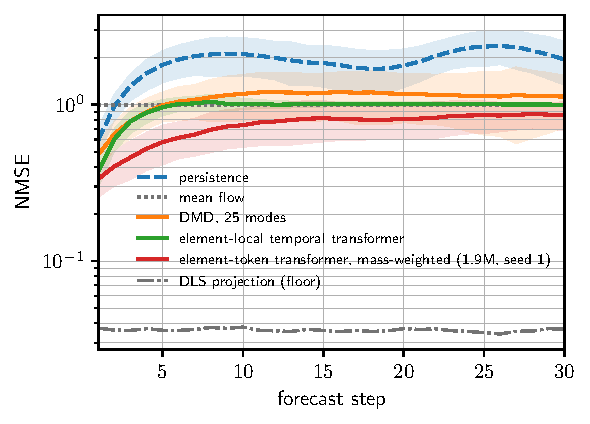
\includegraphics[width=0.6\textwidth]{challenge_heldout.pdf}
  \caption{Challenge 2.1 forecast error on 30 held-out sequences: official NMSE on the full grid; lines are means over sequences and bands are $\pm$ one standard deviation. The element-token transformer (1.9 million parameters, mass-weighted projection in the loop) stays below the mean-flow forecast at every lead time.}
  \label{fig:challenge}
\end{figure}

\subsection{Forecast error and fluctuation recovery}
\label{sec:tradeoff}
The Challenge 2.1 forecasts lose amplitude as they lose skill, and NMSE rewards this. The reason is exact. For one sequence at lead $k$, let $E_k=\|\hat{\mathbf{q}}_k\|^2/\|\mathbf{q}_k\|^2$ be the energy ratio of the mean-removed forecast and $c_k=\langle\hat{\mathbf{q}}_k,\mathbf{q}_k\rangle/(\|\hat{\mathbf{q}}_k\|\,\|\mathbf{q}_k\|)$ its pattern correlation with the truth. Then
\begin{equation}
  \mathrm{NMSE}_k=1+E_k-2c_k\sqrt{E_k}=1-c_k^2+\bigl(c_k-\sqrt{E_k}\bigr)^2 .
  \label{eq:nmse_id}
\end{equation}
This is Murphy's decomposition of the mean-square-error skill score \cite{murphy1988skill}, and the law of cosines behind the Taylor diagram \cite{taylor2001diagram}. For a given correlation, the NMSE is smallest when the forecast carries the energy $E_k=c_k^2$, and the minimum is $1-c_k^2$. A forecast with the true energy scores $2(1-c_k)$. This exceeds the mean-flow value of 1 whenever $c_k<1/2$, however realistic the forecast's statistics.

The deterministic models are close to this optimum. Over three seeds of the 1.9-million-parameter model (on the variant of the basis described below, with $\alpha=0.1$), the correlation falls from 0.81 at the first step to 0.52 at step 10 and 0.32 at step 30. Over the same steps the energy ratio falls from 0.68 to 0.35 and 0.18, tracking $c_k^2$ (0.66, 0.27, 0.10). Averaged over sequences and steps, the correlation term $1-c_k^2$ accounts for 0.718 of the mean NMSE of 0.765. The amplitude term accounts for the remaining 0.047: 0.002 at the first step and at most 0.069 at any lead. A model trained on a mean-square loss approximates the conditional mean of the future state, and Eq.~\eqref{eq:nmse_id} shows what this implies for amplitude. Its loss of energy is the NMSE-optimal response to its own correlation, not a failure of training. The NMSE can then be lowered appreciably only by raising the correlation, and energy can be recovered at fixed correlation only by raising the NMSE.

The same identity gives a baseline for any method that claims to recover fluctuations. Multiplying a forecast by a lead-dependent gain $g_k$ scales $E_k$ by $g_k^2$ and leaves $c_k$ unchanged. It therefore moves the forecast along Eq.~\eqref{eq:nmse_id} without adding information. We take $g_k=\bar E_k^{-\theta/2}$, where $\bar E_k$ is the model's mean energy ratio on seven sequences from the test block (starting at snapshots 10,800--11,400), and vary $\theta$. With $\theta=0$ the forecast is unchanged, and $\theta=1$ restores the true energy on those seven sequences. Averaged over the three seeds, the rescaled forecasts trace a curve of NMSE against energy, which serves as the reference. A change of loss, basis, or tokenization adds information only if it lands below this curve. For each configuration we therefore report $\Delta_g$, its NMSE minus that of the rescaled reference at the same energy.

Table~\ref{tab:tradeoff} applies this baseline and the statistics of Sec.~\ref{sec:eval} to the configurations studied so far, each trained with three seeds. The seed-to-seed variation in NMSE is substantial. The 30-step mean NMSE of the reference recipe spans 0.742--0.789, so differences below about 0.05 between the single runs of Table~\ref{tab:challenge} are not significant.

The variant with $\alpha=0.1$ changes how the cut elements of the full-coverage mesh are fitted (Sec.~\ref{sec:fullcover}). Instead of carrying zero weight, the grid points outside the domain are fitted, with weight 0.1, to an odd reflection of the field about the boundary. This changes nothing measurable. Doubling the enrichment from five to ten modes per node brings the basis closer to the truth in every statistic, most visibly in the spatial spectrum, where its distance falls from 17.8 to 11.9 times the floor. The forecasts do not use the richer space: their NMSE, correlation, energy, and statistics match the five-mode model's within the seed spread, and $\Delta_g$ is slightly positive. The free rollouts of every deterministic configuration are far from the true flow, at 52--55 times the floor in spectral shape and 4.7--4.8 times in distribution shape. The DLS projections are within the floor except for the spatial spectrum, where the finite enrichment removes the smallest scales. The gap between the forecasts and their basis is therefore set by the training objective, not by the representation.

To move a deterministic model along the curve by training rather than by a gain, we add to the loss a term that penalizes the error in each frame's field energy, $\beta\,(\|\hat{\mathbf{u}}\|-\|\mathbf{u}\|)^2$, computed with $\lambda=0$ in Eq.~\eqref{eq:loss}. For a forecast whose only freedom is its amplitude, the combined loss is smallest at $\sqrt{E}=(c+\beta)/(1+\beta)$. This interpolates between the NMSE optimum ($\beta=0$) and the true energy ($\beta\rightarrow\infty$). Computed instead in the regularized metric, whose norm is mostly ridge (Sec.~\ref{sec:gram}), the term matched an energy that the model cannot predict and inflated the visible field: the forecasts carried 1.5 and 2.5 times the true energy at $\beta=1$ and 3.

With $\lambda=0$ the term behaves as the per-frame analysis predicts (Table~\ref{tab:tradeoff}; one seed each). For $\beta=0.1$, 0.3, 1, and 3, the 30-step forecasts carry 0.37, 0.43, 0.64, and 0.75 of the true energy. The values predicted from their own correlations are 0.35, 0.40, 0.56, and 0.75, and the correlation stays at 0.46--0.51. The NMSE rises from 0.74 to 0.97. $\Delta_g$ lies between $-0.03$ and $+0.04$, within the spread of the reference's own seeds ($-0.03$ to $+0.03$). The term therefore moves the model along the rescaled curve, as a gain would, without adding information. Over the free rollout it restores amplitude. For $\beta\geq1$ the energy ratio rises to 0.71, and the RMS-map error falls from 8 times its floor to 4--5.5 times. How that energy is distributed improves much less. The spectral shapes remain 32--59 times their floors and the distribution shape 3.6--4.7 times, against 54--55 and 4.8 for the reference. The largest change is in the frequency spectrum at $\beta=3$, from 54 to 32 times its floor, and that model's NMSE is 0.97. An energy constraint can thus restore how much a deterministic forecast fluctuates, but it changes little about how. \todo{Seeds for one $\beta$; a figure of NMSE against energy with the gain curve.} \todo{Tokenization sweep (patch size at a fixed number of coefficients). Decide whether the stochastic hybrid enters this paper.}

\begin{table}[!tbp]
  \centering
  \small
  \setlength{\tabcolsep}{3pt}
  \caption{Forecast error and fluctuation recovery on Challenge 2.1, 1.9 M model, three seeds unless noted (mean $\pm$ standard deviation, or mean). Left: 30-step forecasts of the 30 held-out sequences, with mean NMSE over steps 1--30, energy ratio $E$, pattern correlation $c$, and $\Delta_g$, the NMSE minus that of the rescaled $\alpha=0.1$, five-mode reference at the same energy (negative is better than a gain). Right: free rollout over the held-out block (Sec.~\ref{sec:eval}), with the fluctuating-energy ratio and the other distances as multiples of their sampling floors (RMS map 0.072; spatial and frequency spectrum shape 0.30 and 0.37~dB; distribution shape 0.054).}
  \label{tab:tradeoff}
  \begin{tabular}{lccccccccc}
    \toprule
    & \multicolumn{4}{c}{30-step forecasts} & \multicolumn{5}{c}{Free rollout} \\
    \cmidrule(lr){2-5}\cmidrule(lr){6-10}
    Configuration & NMSE & $E$ & $c$ & $\Delta_g$ & Energy & RMS map & $x$ spectrum & $t$ spectrum & PDF \\
    \midrule
    True flow, other segments & -- & -- & -- & -- & 0.96 & 1 & 1 & 1 & 1 \\
    DLS projection, 5 modes & -- & -- & -- & -- & 0.97 & 0.3 & 17.8 & 0.7 & 0.3 \\
    DLS projection, 10 modes & -- & -- & -- & -- & 0.98 & 0.2 & 11.9 & 0.5 & 0.3 \\
    \midrule
    5 modes, $\alpha=0$ & $0.775\pm0.004$ & $0.30\pm0.04$ & 0.46 & $+0.01$ & $0.17\pm0.01$ & 8.7 & 54 & 52 & 4.7 \\
    5 modes, $\alpha=0.1$ (reference) & $0.765\pm0.023$ & $0.30\pm0.03$ & 0.47 & $0.00$ & $0.21\pm0.02$ & 8.1 & 55 & 54 & 4.8 \\
    10 modes, $\alpha=0.1$ & $0.785\pm0.019$ & $0.28\pm0.02$ & 0.45 & $+0.02$ & $0.20\pm0.06$ & 8.4 & 53 & 52 & 4.7 \\
    \midrule
    \multicolumn{10}{l}{\emph{Reference with the energy term, $\lambda=0$, one seed:}} \\
    \quad $\beta=0.1$ & 0.744 & 0.37 & 0.51 & $-0.03$ & 0.30 & 7.5 & 56 & 54 & 4.7 \\
    \quad $\beta=0.3$ & 0.781 & 0.43 & 0.48 & $-0.02$ & 0.41 & 6.2 & 59 & 50 & 4.7 \\
    \quad $\beta=1$ & 0.879 & 0.64 & 0.47 & $0.00$ & 0.71 & 4.0 & 58 & 40 & 4.3 \\
    \quad $\beta=3$ & 0.967 & 0.75 & 0.46 & $+0.04$ & 0.71 & 5.5 & 49 & 32 & 3.6 \\
    \bottomrule
  \end{tabular}
\end{table}

%=====================================================================================
\section{Discussion}
\label{sec:discussion}
The results support treating the data-enriched finite element basis as more than a compressor. The element structure supplies the tokens, and the forecast is posed on local, position-aware units that share one set of weights. The mass matrix supplies the metric. Scoring in the raw coefficient metric would weight directions that carry almost no field energy, and the same correction makes POD on the latent exact. For training, the metric needs a ridge to keep rollouts stable. On an ill-conditioned basis that ridge carries most of the loss, so terms meant for the visible field must be computed without it. The assembly operator supplies consistency. Combining element predictions by the field-metric projection improved every short-horizon metric in every seed, and training through that projection improved the 30-step error and its consistency across seeds. None of these components uses the governing equations; the forecast remains purely data-driven. The finite element structure acts on the forecast only through the geometry of the latent space.

The same recipe transferred to experimental data without changes to the architecture. On the Challenge 2.1 cavity it is the only model tested whose error stays below that of the mean-flow forecast throughout the 30-step window. Its pattern correlation with the truth stays well above DMD's at every lead time. Two lessons from the cavity concern capacity. Narrower networks forecast as well as the full one, and a longer stacked input history makes the model overfit within a few epochs. The record contains less information that generalizes than the full network can absorb, so capacity is better spent on the spatial structure of the element tokens than on per-token detail.

Three limitations stand out. First, higher compression moves the error budget from the forecast to the representation: with five modes per node, the RMS error is within one point of a floor that is itself 8.8\%. The choice of basis should therefore be made with the downstream statistic in mind. A richer basis is not enough on its own, however. On Challenge 2.1, ten modes per node brought the basis closer to the true statistics without changing the forecasts, so more enrichment pays off only with a training objective that makes use of it. Second, at $\Rey=30{,}000$ the limiting factor is the amount and stationarity of the training record rather than the architecture. More data was the only change that improved the forecast (skill from 0.02 to 0.33), whereas weight decay and input noise did not help. Third, a deterministic model trained on a mean-square loss converges toward the conditional mean of the future state. Where predictability is short, as in the Challenge 2.1 cavity and at $\Rey=30{,}000$, its forecasts lose amplitude as they lose skill (18\% and 65\% of the true fluctuating energy over the long rollouts). Section~\ref{sec:tradeoff} shows that this loss of energy is the NMSE-optimal response to the forecast's own correlation. NMSE therefore rewards it, but turbulence statistics do not: on Challenge 2.1 the free rollouts are about 50 times the sampling floor in spectral shape. Generative or stochastic forecasting on the same element tokens \cite{kohl2023acdm,lippe2023pderefiner} is the natural way to keep both.

%=====================================================================================
\section{Conclusions}
\label{sec:conclusions}
We posed transformer forecasting of turbulent flow on the elements of a data-enriched finite element basis, with one token per element and attention over space. On the lid-driven cavity at $\Rey=15{,}000$, with 2,662 latent coefficients (four times fewer than our prior work), the model forecasts 30 steps ahead with a mean relative field error of 3.8\%, against 32.4\% for persistence. The error is consistent across forecasts and across seeds, and its 500-step RMS velocity field is within 1.4 percentage points of the compression floor. Two finite element ingredients were responsible for much of the improvement over the original formulation: a field-energy metric from the basis's mass matrix, and a mass-weighted projection of the element predictions, applied inside the training rollout. Attention over element tokens outperformed a global temporal transformer on the same latent space. A fictitious-domain extension of the mesh lets the same basis represent grids whose size is not a multiple of the element size. At $\Rey=30{,}000$ the recipe overfits a short training record; a longer record raises the 30-step skill to 0.33, but the long rollout still loses energy. On the Challenge 2.1 cavity PIV, a 1.9-million-parameter version of the model has a mean 30-step NMSE of 0.78 on held-out sequences, against 1.09 for the DMD baseline and 1.0 for the mean flow, with a pattern correlation that stays well above DMD's at every lead time. The remaining gap is amplitude: the forecasts damp toward the mean as predictability is lost.

\section*{Acknowledgments}
This project is supported by the Office of Naval Research under grant number N00014-23-1-2398, with Leighton Meyers as Program Officer. The authors acknowledge the use of DoD HPCMP computing resources. The authors also thank Dr. Sachin Kumar for helpful discussions and insights on this work. \todo{The abstract also thanked Ryan Czerwiec (NAVAIR) for the airwake data; drop or keep depending on whether any airwake material remains.}

\bibliography{references}

\end{document}
